\documentclass[conference]{IEEEtran}
\usepackage{amsmath,amssymb,amsfonts}
\usepackage{graphicx}
\usepackage{textcomp}
\usepackage{booktabs}
\usepackage{multirow}
\usepackage{url}
\usepackage{xcolor}
\usepackage{subcaption}
\usepackage{amsthm}
\newtheorem{proposition}{Proposition}

\def\BibTeX{{\rm B\kern-.05em{\sc i\kern-.025em b}\kern-.08em
    T\kern-.1667em\lower.7ex\hbox{E}\kern-.125emX}}

\begin{document}

\title{Won by a Single Question:\\Item-Level Attribution and the Robustness of LLM Leaderboard Decisions}

\author{\IEEEauthorblockN{Utkarsh Bajaj and Madhur Mehta}
\IEEEauthorblockA{\textit{Independent Researchers}\\
\texttt{\{utkarshbajaj2401,themadhurmehta\}@gmail.com}}}

\maketitle

\begin{abstract}
Public leaderboards rank large language models by aggregate benchmark scores, but a model-selection decision may rest on only a few individual items.
We introduce \emph{Decision-Shapley}, a framework that attributes a particular adjacent-model ranking to benchmark items.
We show that two natural value functions are degenerate: the score margin reduces Shapley to leave-one-out, while a binary flip indicator reduces it to the Shapley--Shubik power index and treats all same-direction items alike.
We therefore develop a correlation-aware confidence value function and a Fisher-weighted information value function that distinguish items through redundancy and discrimination.
Across 90 adjacent-rank contests on LiveBench and the Open~LLM~Leaderboard~v1, 58 have an item-bootstrap flip probability above 30\%; the leading model on LiveBench's \texttt{LCB\_generation} task has a net margin of one item out of 78.
A value-function-free analysis finds no evidence that global Item Response Theory discrimination predicts local decisiveness beyond mechanical coupling, showing that global informativeness and decision-specific leverage are distinct.
Decision-Shapley complements uncertainty and benchmark-validity analyses: it identifies items to inspect, not items that are intrinsically good or bad.
We implement the analysis in a report-card tool for per-item binary result matrices.
\end{abstract}

\begin{IEEEkeywords}
LLM evaluation, leaderboard robustness, Shapley values, power indices, benchmark attribution, decision analysis
\end{IEEEkeywords}

%======================================================================
\section{Introduction}
\label{sec:intro}
%======================================================================

Public leaderboards have become the de facto mechanism by which practitioners select large language models (LLMs).
A model's aggregate score, the mean over hundreds or thousands of test items, determines its rank, and the top-ranked model is taken as ``the best.''
Decisions of considerable practical consequence (which model to deploy, which API to integrate, which foundation to fine-tune) flow directly from these rankings.
Yet aggregate scores obscure a critical question: \emph{how many individual test items does the selection of the winner actually depend on, and which ones?}

Consider a concrete case from our analysis.
On the \texttt{LCB\_generation} task of LiveBench~\cite{livebench}, whose coding problems are drawn from the separate LiveCodeBench benchmark~\cite{jain2024livecodebench}, Gemini~2.5~Pro ranks \#1 with a score of 89.7\%, just above QwQ-32B at 88.5\%.
This gap corresponds to a \emph{net margin of exactly one item} out of 78: Gemini answers 4 questions correctly that QwQ misses, while QwQ answers 3 that Gemini misses.
The remaining 71 items, 91\% of the benchmark, are redundant for this decision because both models answer them identically.
Bootstrap resampling reveals a 42.5\% probability that this ranking would reverse under a different draw of test items.
The ranking is therefore highly sample-sensitive under this resampling model; this is not a posterior probability that the reported winner is wrong.

This fragility is not an anomaly.
Across all 90 rank-boundary contests we analyze on two benchmark suites, 58 (64\%) have bootstrap flip probabilities exceeding 30\%, and 72 (80\%) exceed 10\%.
That leaderboard rankings can be unstable is itself not new~\cite{alzahrani2024benchmarks, miller2024adding}; the open question is \emph{which specific items} a decision rests on, and how to attribute responsibility to them in a principled way.

Doing this correctly is subtle, and the subtlety is the heart of our contribution.
Casting the contest as a cooperative game and computing Shapley values is the natural move, but the result depends entirely on the value function, and the two obvious choices both \emph{degenerate}: an additive margin function makes Shapley collapse to leave-one-out, while a binary flip-indicator function makes it collapse to the Shapley--Shubik power index~\cite{shapleyshubik1954}, under which every item with the same differential is an interchangeable ``voter'' and there is no per-item signal.
A method built on either cannot, even in principle, say one decisive item matters more than another.
We resolve this with two non-degenerate value functions that break the symmetry through statistical structure (item correlation and discrimination), with the degenerate case as their formal special limit.

Separately, we ask whether a standard global item statistic, Item Response Theory (IRT) discrimination / Fisher information~\cite{kipnis2025metabench, polo2024tinybenchmarks}, already predicts which items are decisive.
If it did, decision-specific attribution would be unnecessary.
Through a value-function-free validation against a mechanical-coupling null, we find that it does \emph{not}: global discrimination and local decisiveness are distinct properties.
This negative result is the empirical justification for the method.

\textbf{Contributions.} We make four contributions:

\begin{enumerate}
    \item \textbf{Framework.} Decision-Shapley, which attributes a specific pairwise leaderboard decision (\#$k$ vs.\ \#$k\!+\!1$) to individual items, with the unit of analysis being the \emph{decision}, not the ranking (\S\ref{sec:method}).
    \item \textbf{Non-degenerate value functions.} A correlation-aware confidence value function with a conditional probabilistic interpretation, which splits credit among redundant items, plus a Fisher-weighted information value function, with Proposition~\ref{prop:degeneracy} showing the flip indicator is the degenerate Shapley--Shubik special case (\S\ref{sec:value}).
    \item \textbf{Empirical audit.} A 90-contest audit separates decision fragility from item attribution and tests whether global IRT discrimination predicts local decisiveness beyond mechanical coupling (\S\ref{sec:experiments}).
    \item \textbf{Artifact.} A report-card tool: input any per-item binary result matrix $\to$ output a decision-robustness report (\S\ref{sec:reportcard}).
\end{enumerate}

%======================================================================
\section{Related Work}
\label{sec:related}
%======================================================================

Prior work asks three adjacent but distinct questions: whether rankings are stable, which items are globally informative, and how credit is assigned within a decision.
We connect these strands while keeping robustness measurement and item attribution distinct.

\subsubsection{Leaderboard Stability}
Ranking uncertainty is well established, but prior work stops short of item-level attribution.
Alzahrani et al.~\cite{alzahrani2024benchmarks} study global stability under item perturbation; Miller~\cite{miller2024adding} adds confidence intervals to leaderboard gaps; and Burnell et al.~\cite{burnell2023rethink} and Card et al.~\cite{card2020power} motivate uncertainty and power analysis.
We instead condition on one adjacent-model decision and identify the items on which it rests.

\subsubsection{Benchmark Redundancy and IRT}
IRT and low-rank methods compress benchmarks or select efficient subsets~\cite{kipnis2025metabench,polo2024tinybenchmarks,fromskills2024,perlitz2024efficient}.
They identify \emph{globally informative} items; we identify items \emph{decisive for one realized contest}, and show the notions do not coincide (\S\ref{sec:extval}).

\subsubsection{Cooperative Game Theory and Power Indices}
Shapley~\cite{shapley1953value} introduced the value for cooperative games; Shapley--Shubik~\cite{shapleyshubik1954} specialized it to weighted voting.
The Banzhaf index~\cite{banzhaf1965} is a swing count: the fraction of coalitions for which adding an item changes the decision.
SHAP~\cite{lundberg2017shap} attributes model outputs to features, while data-Shapley~\cite{ghorbani2019data,jia2019efficient} values training data.
Our players are benchmark items and our coalition scores are nonlinear and structure-aware (\S\ref{sec:value}).

\subsubsection{LLM Evaluation Methodology}
HELM~\cite{liang2023helm} remains score-aggregated, whereas Chatbot Arena~\cite{zheng2024chatbot} uses pairwise human comparison.
Our framework applies to either setting; we instantiate benchmark contests and leave vote-level attribution to future work.

In short, existing methods measure stability, global informativeness, or game-theoretic credit; none jointly localizes a signed pairwise decision while accounting for redundancy.

%======================================================================
\section{Method}
\label{sec:method}
%======================================================================

\subsection{Setup}
\label{sec:setup}

Let $R \in \{0,1\}^{M \times N}$ be a per-item binary response matrix for a benchmark with $M$ models and $N$ items, where $R_{m,i} = 1$ if model $m$ answers item $i$ correctly, and let $\text{score}(m) = \frac{1}{N}\sum_{i} R_{m,i}$.
For a rank boundary $k$, let $m_1$ be the model at rank $k$ and $m_2$ at rank $k\!+\!1$, with $\text{score}(m_1) > \text{score}(m_2)$.
For each item $i$, define the \emph{per-item differential}
\begin{equation}
    d_i = R_{m_1, i} - R_{m_2, i} \in \{-1, 0, +1\},
    \label{eq:differential}
\end{equation}
and the \emph{margin} $\Gamma = \sum_{i} d_i > 0$.
Items partition into three groups: $d_i = +1$ (favor $m_1$, count $n_+$), $d_i = -1$ (favor $m_2$, count $n_-$), and $d_i = 0$ (neutral, count $n_0$), with $\Gamma = n_+ - n_-$.
Items with $d_i = 0$ carry \emph{no} information about the pairwise decision yet may constitute the vast majority of the benchmark (e.g., 91\% on \texttt{LCB\_generation}).

\subsection{Value Functions and a Degeneracy}
\label{sec:value}

The central design choice is the value function $v: 2^{[N]} \to \mathbb{R}$ over item coalitions, from which item Shapley values $\phi_i$ are derived in the usual way.
Conceptually, a coalition is a subset of benchmark items, $v(S)$ summarizes how strongly that subset supports the observed winner, and Shapley attribution averages how much each item changes that support when added to many possible subsets.
The goal is not merely to identify items that change the raw score, but to separate unique evidence from evidence that is redundant with other items.
We consider four value functions: two natural but degenerate choices establish the problem, and two structure-aware choices provide genuine per-item attribution.

\subsubsection{Margin (Additive)} $v_{\text{margin}}(S) = \sum_{i \in S} d_i$.
By linearity each item's Shapley value equals $d_i$ regardless of the others: Shapley reduces exactly to leave-one-out (LOO), and the credit-splitting benefit of cooperative game theory disappears.

\subsubsection{Flip Indicator}
\begin{equation}
    v_{\text{flip}}(S) = \begin{cases}
        1 & \sum_{i \in S} d_i > 0 \\
        \tfrac12 & \sum_{i \in S} d_i = 0 \\
        0 & \sum_{i \in S} d_i < 0
    \end{cases}
    \label{eq:value}
\end{equation}
with $v(\emptyset) = \tfrac12$.
This is nonlinear and was, in an earlier version of this work, the value function we used.
It has an important and previously unrecognized limitation: it depends on the coalition only through $\sum_{i\in S} d_i$, so \emph{all items sharing the same $d_i$ are symmetric players}.
The game is exactly a weighted voting game with weights $d_i$, and its Shapley values are the Shapley--Shubik power index~\cite{shapleyshubik1954}.
Consequently there are only three distinct Shapley values per contest (one each for $d_i=+1,-1,0$); any observed variation \emph{within} a group is Monte-Carlo noise, not signal.
Genuine per-item attribution is therefore impossible under $v_{\text{flip}}$.

\subsubsection{Confidence (Correlation-Aware)}
We want $v(S)$ to quantify how strongly coalition $S$ supports the observed winner while accounting for overlap among its items.
We obtain a model-based confidence score from an explicit Gaussian evidence model rather than positing a convenience heuristic.
Let $w_i = a_i d_i$, where $a_i$ is item $i$'s discrimination (the point-biserial correlation of item $i$ with total score, a classical test-theory quantity~\cite{lordnovick1968}) and $d_i$ its realized direction, so $w_i$ is the discrimination-weighted vote item $i$ casts toward the winner.
Let the coalition's observed net evidence be $T_S=\sum_{i\in S} w_i=\mu_S$.
Under the working likelihood $T_S\mid\delta_S\sim\mathcal{N}(\delta_S,\sigma_S^2)$, where $\delta_S$ is the coalition's latent net evidence and $\sigma_S=\sqrt{w_S^\top C_S\,w_S}$ uses the empirical item-correlation matrix $C_S$, a flat prior on $\delta_S$ yields
\begin{equation}
    v_{\text{conf}}(S) = \Phi\!\left(\frac{\mu_S}{\sigma_S}\right),\quad
    \mu_S = \sum_{i\in S} w_i,\quad
    \sigma_S^2 = w_S^\top C_S\, w_S,
    \label{eq:conf}
\end{equation}
with $\Phi$ the standard normal CDF and $v(\emptyset)=\tfrac12$.
Thus $v_{\text{conf}}$ has a posterior interpretation only conditional on the Gaussian likelihood, flat prior, and plug-in estimates of $a_i$ and $C_S$; we do not claim that it is an empirically calibrated probability across arbitrary benchmarks.
Three properties pin down how the score behaves.
First, in the degenerate limit of Proposition~\ref{prop:degeneracy} (equal discrimination, $C=I$, hard threshold) it collapses to the exact indicator $\mathbf{1}[\sum_{i\in S} d_i>0]$, i.e.\ ``does coalition $S$ flip the decision,'' so $v_{\text{conf}}$ is the correlation-aware generalization of that exact event.
Second, because $\sigma_S$ accounts for redundancy, two highly correlated decisive items split the credit a single independent item would receive.
Third, the model has a limited scope, which matters for the validation in \S\ref{sec:e18val}: since $\Phi(\mu_S/\sigma_S)$ standardizes by $\sigma_S$, the overall scale of the weights cancels and a singleton is worth $\Phi(\pm1)$ whatever $a_i$ is.
Confidence thus reads item correlation but is blind to per-item discrimination magnitude.
It is the appropriate correlation-aware score when the active items are about equally informative; once a contest turns on items of very different discrimination, the model no longer fits, and the information value function below is the one to use.

\subsubsection{Information (Fisher-Weighted)}
The confidence model weights every active item equally up to sign and correlation; a complementary model weights each item by how sharply it discriminates.
Let $J_i$ be item $i$'s 2PL Fisher information at the contest ability midpoint $\theta^\star=\tfrac12(\theta_{m_1}+\theta_{m_2})$, i.e.\ $J_i=a_i^2\,p_i^\star(1-p_i^\star)$ with $p_i^\star$ the success probability at $\theta^\star$, and let $C_S$ be the Ledoit--Wolf-shrunk $\phi$-coefficient correlation of the active items in $S$.
Treat each active item as a noisy measurement of one common ``winner leads'' signal whose precision is its discrimination $J_i$; stacking these measurements gives a generalized least squares (GLS) problem with covariance $\Sigma_S=D_S\,C_S\,D_S$ and $D_S=\operatorname{diag}(J_i^{-1/2})$.
The GLS estimate of the common signal, standardized by its own standard error, is
\begin{equation}
    v_{\text{info}}(S)=\Phi(z_S),\qquad
    z_S=\frac{d_S^{\top}\,\Sigma_S^{-1}\,\mathbf{1}}{\sqrt{\mathbf{1}^{\top}\,\Sigma_S^{-1}\,\mathbf{1}}},
    \label{eq:info}
\end{equation}
with $d_S$ the realized item directions, $\mathbf{1}$ the all-ones vector, and $v(\emptyset)=\tfrac12$.
Equivalently, writing $g_i=\sqrt{J_i}$, $h_i=d_i\sqrt{J_i}$, and $y_S=C_S^{-1}g_S$, we have $z_S=(h_S^{\top}y_S)/\sqrt{g_S^{\top}y_S}$, which is what we compute (one linear solve per coalition).
Unlike $v_{\text{conf}}$, the discrimination scale does \emph{not} cancel: a singleton is worth $\Phi(\pm\sqrt{J_i})$, increasing in $J_i$, so higher-discrimination items receive strictly higher attribution (verified by exact computation, \S\ref{sec:e1}).
Like $v_{\text{conf}}$, it reduces to the flip indicator under equal discrimination, $C=I$, and a hard threshold, so Proposition~\ref{prop:degeneracy} covers it as well.

\begin{proposition}[Degeneracy]
\label{prop:degeneracy}
If (a) all items have equal discrimination $a_i=a$, (b) the correlation matrix is the identity $C=I$, and (c) $\Phi$ is replaced by the hard step $\mathbf{1}[x>0]$, then $v_{\text{conf}}$ reduces to the flip indicator $v_{\text{flip}}$, and the Decision-Shapley values reduce to the Shapley--Shubik power index.
\end{proposition}
\begin{proof}[Proof sketch]
With $w_i = a\,d_i$ and $C=I$, $\sigma_S^2 = a^2\sum_{i\in S} d_i^2 = a^2 |S_{\text{act}}|$, so the argument of $\Phi$ is $(a\sum d_i)/(a\sqrt{|S_{\text{act}}|}) = (\sum d_i)/\sqrt{|S_{\text{act}}|}$.
Under a hard step this is $1$ iff $\sum d_i>0$, $0$ iff $<0$, and $\tfrac12$ at $0$, exactly $v_{\text{flip}}$.
The voting game's Shapley values are the Shapley--Shubik index by definition~\cite{shapleyshubik1954}.
\end{proof}

Proposition~\ref{prop:degeneracy} both explains the earlier degeneracy and positions the confidence value function as a principled generalization: discrimination and correlation are exactly the two ingredients the flip indicator discards.

\subsubsection{Choosing Between the Two Decision Models}
Confidence and information are two decision models with different assumptions, an equal-informativeness correlation-aware model and a discrimination-weighted one, rather than a primary tool and a backup; which one fits is decided by the spread of active-item discriminations, which is observable.
Confidence applies when the active items are comparably discriminating, and information when they differ substantially; our tool computes both and reports the spread.
We checked this rule rather than assuming it: \S\ref{sec:e18val} shows each value function is the better estimator of the true decision where it is well-specified.
We report confidence by default because it expresses standardized support under a transparent working model, and the homogeneous regime, where redundancy rather than discrimination separates items, is typical of the saturated, converged contests where selection is most fragile.

\subsection{Monte Carlo Estimation}
\label{sec:mc_shapley}

We estimate $\phi_i$ by permutation sampling.
For the flip indicator, a permutation walk maintains a running sum $g$ and records each item's marginal change in $v$; items with $d_i=0$ have zero marginal in every permutation, so $\phi_i=0$ exactly.
For the confidence value function we maintain a running signal $\mu$ and variance $\sigma^2$ with an $O(|S|)$ update per step.
The information value function instead solves the GLS system of Eq.~\ref{eq:info} on the coalition's correlation submatrix, $O(|S|^3)$ per coalition, which is inexpensive in practice because the active sets of real contests are small.
We use $T=20{,}000$ permutations, achieving max SE $<0.002$; an exact brute-force solver cross-validates the estimator on small contests.

\subsection{Bootstrap Flip Probability}
\label{sec:bootstrap}

Decision fragility is measured independently of the value function by resampling the $N$ items with replacement $B=50{,}000$ times, recomputing $\Gamma^*=\sum d_{i^*}$, and reporting $P(\Gamma^*\leq 0)$ with a Wilson interval~\cite{efron1979bootstrap}.
This estimates sensitivity to a different draw from a \emph{superpopulation}, the hypothetical population of equally valid items produced by the same benchmark-construction process.
It is conditional on the item-exchangeability model and is not the probability that the reported winner is wrong.
Because it depends only on $d$, it is robust to any value-function choice, so the fragility findings of \S\ref{sec:fragility} stand regardless of the Shapley debate above.

\subsection{Item Taxonomy}
\label{sec:taxonomy}

Relative to the realized model pair, we classify each item as \emph{decisive} ($\phi_i>0$, always $d_i=+1$), \emph{counter-evidential} ($\phi_i<0$, always $d_i=-1$; the runner-up outperforms the winner here), or \emph{decision-redundant} ($\phi_i\approx 0$, including all $d_i=0$ items).
Decision-redundant does not mean globally uninformative or removable from the benchmark; the item may distinguish other models or contribute to construct coverage.
Counter-evidential items are invisible to unsigned global metrics but surfaced directly by signed Shapley attribution.

%======================================================================
\section{Experiments}
\label{sec:experiments}
%======================================================================

\subsection{Degeneracy and Symmetry-Breaking (E1)}
\label{sec:e1}

We validate the value-function analysis on controlled synthetic matrices with exact (brute-force) Shapley values.
First, margin-based Shapley assigns $\phi_i=d_i$ to every item, identical to LOO, confirming the additive degeneracy.
Second, under the flip indicator, three decisive items with \emph{different} discriminations $a=(2.0,0.5,1.0)$ but identical $d_i=+1$ receive identical Shapley values (the Shapley--Shubik symmetry).

Confidence breaks this symmetry through correlation, not discrimination: with $C=I$ the three items receive $\phi\approx(0.142,0.142,0.153)$, so discrimination is a weak, non-monotonic lever (a singleton is worth $\Phi(\pm1)$, scale-invariant), while redundancy is the robust one (two items correlated at $0.95$ earn $\approx0.125$ each versus $\approx0.16$ when independent, splitting credit as cooperative game theory should).
Information, by contrast, makes discrimination monotonic: higher-$J$ items receive strictly higher $\phi$ (verified exactly).
These are the two decision models of \S\ref{sec:value}.

\subsection{Datasets}
\label{sec:datasets}

\subsubsection{LiveBench}
LiveBench~\cite{livebench} is a contamination-resistant benchmark with verifiable ground truth.
Contamination here means benchmark items leaking into a model's training data, which would inflate its score without reflecting genuine ability; LiveBench resists this by drawing questions from recently released sources (math competitions, papers, news) dated after the models' training cutoffs, so the items are unlikely to have been seen during training.
We note this property belongs to the benchmark, not to individual models.
We use the \texttt{model\_judgment} data (March 2025) with per-question binary scores for 58--155 models across three fully binary tasks: \texttt{LCB\_generation} (78 items), \texttt{coding\_completion} (50 items), and \texttt{typos} (100 items).
The \texttt{LCB\_generation} task draws its coding problems from the separate LiveCodeBench benchmark~\cite{jain2024livecodebench}; throughout we analyze the version packaged and scored within LiveBench, and reserve the name ``LiveCodeBench'' for Jain et al.'s benchmark.
Models include Gemini~2.5~Pro, o3-mini, GPT-4.5~Preview, Claude~3.7~Sonnet, DeepSeek~R1, and QwQ-32B.

\subsubsection{Open LLM Leaderboard v1}
The Open LLM Leaderboard v1 (via Polo et al.~\cite{polo2024tinybenchmarks} / metabench~\cite{kipnis2025metabench}) provides full per-item binary matrices for six benchmarks over the complete leaderboard release (5{,}225--6{,}702 models per benchmark across $\approx$29{,}000 items): ARC (1{,}172 items), GSM8K (1{,}319), HellaSwag (10{,}042), MMLU (14{,}042), TruthfulQA (817), and WinoGrande (1{,}267).
These are community fine-tunes and merges from 2023--2024; the benchmarks are now saturated, and the top-ranked checkpoints are frequently obscure models for which contamination cannot be excluded (the top TruthfulQA model scores 100\%).
We therefore treat the Open~LLM data as a large-scale methodological testbed representative of real leaderboard practice, and rely on LiveBench for the contamination-resistant frontier view.

\subsection{Decision Fragility Across Rank Boundaries}
\label{sec:fragility}

Table~\ref{tab:top1} shows the \#1~vs.~\#2 contests.
The frontier LiveBench contests are markedly fragile (flip $\geq$ 19\%), whereas the saturated Open~LLM top contests vary widely: ARC and MMLU are robust (flip $\approx$ 0, with comfortable item margins), while GSM8K and WinoGrande are tighter.
ARC, with a 7.59-percentage-point top-2 gap, is our deliberate \emph{robust} reference, not a fragility example.

\begin{table}[t]
\centering
\caption{Top-1 vs.\ Top-2 contests. Margin is the net item differential $\Gamma$; Flip\,\% is the value-function-independent bootstrap flip probability; Dec./Ctr./Red.\ are the counts of decisive ($d_i\!=\!+1$), counter-evidential ($d_i\!=\!-1$), and redundant ($d_i\!=\!0$) items.}
\label{tab:top1}
\footnotesize
\setlength{\tabcolsep}{4pt}
\begin{tabular}{@{}lrrrrr@{}}
\toprule
\textbf{Benchmark} & \textbf{Margin} & \textbf{Flip\%} & \textbf{Dec.} & \textbf{Ctr.} & \textbf{Red.} \\
\midrule
\multicolumn{6}{@{}l}{\emph{LiveBench (frontier models)}} \\
\texttt{LCB\_generation} & 1 & 42.5 & 4 & 3 & 71 \\
\texttt{coding\_completion} & 2 & 33.5 & 7 & 5 & 38 \\
\texttt{typos} & 5 & 19.3 & 16 & 11 & 73 \\
\midrule
\multicolumn{6}{@{}l}{\emph{Open LLM Leaderboard v1}} \\
ARC & 89 & 0.0 & 151 & 62 & 959 \\
GSM8K & 11 & 4.5 & 25 & 14 & 1280 \\
HellaSwag & 87 & 0.1 & 430 & 343 & 9269 \\
MMLU & 143 & 0.0 & 514 & 371 & 13157 \\
TruthfulQA & 223 & 0.0 & 223 & 0 & 594 \\
WinoGrande & 7 & 0.9 & 8 & 1 & 1258 \\
\bottomrule
\end{tabular}
\end{table}

We extend the analysis to the first ten valid (non-tied) adjacent-rank contests per benchmark, 90 in all across the nine benchmarks (three LiveBench tasks and six Open~LLM benchmarks); for the saturated TruthfulQA these begin at rank~33, where 33 models tie at 100\%.
We stop at ten because the top of the leaderboard is where model-selection decisions are actually made, and ten contests per benchmark span this competitive region without descending into ranks no practitioner consults.
Fig.~\ref{fig:flip_margin} relates item margin to flip probability: contests with margin $\leq 3$ consistently exceed 16\% flip probability, and at margin~1 the average is 45.4\%, indicating high sample sensitivity under the item bootstrap.
Across all 90 contests, 58 (64\%) exceed 30\% flip probability and 72 (80\%) exceed 10\% (median 38.8\%).
All 30 LiveBench contests analyzed exceed 16\% flip probability (24 of 30 exceed 30\%), while on the Open~LLM benchmarks fragility grows with contest depth.
Because the frontier LiveBench tasks have only $N=50$--$100$ items, their individual flip-probability estimates carry the largest sampling uncertainty (the spread of a proportion estimated from $N$ items narrows roughly as $1/\sqrt{N}$); we therefore read these as a fragile-versus-robust verdict rather than to the decimal, and corroborate the frontier picture with the answer-flip perturbation below and with the much larger Open~LLM item pools.

\subsubsection{Robustness to the Resampling Model}
The item bootstrap treats benchmark items as exchangeable draws from a superpopulation.
This is natural for a refreshing benchmark like LiveBench, whose items are sampled from a continually updated stream, but it is an idealization for a fixed, curated set such as the Open~LLM benchmarks, where no superpopulation literally exists.
We therefore also recompute fragility under an \emph{answer-flip} perturbation that assumes no superpopulation: each response independently flips with probability $\epsilon$.
The two procedures agree on the relative fragility ordering across benchmarks (Spearman $\rho\geq0.85$ for $\epsilon\in\{.01,.03,.05,.10\}$), so our fragility conclusions do not depend on item exchangeability; for fixed benchmarks we regard the answer-flip perturbation as the primary check and the item bootstrap as a convenience.

\begin{figure}[t]
    \centering
    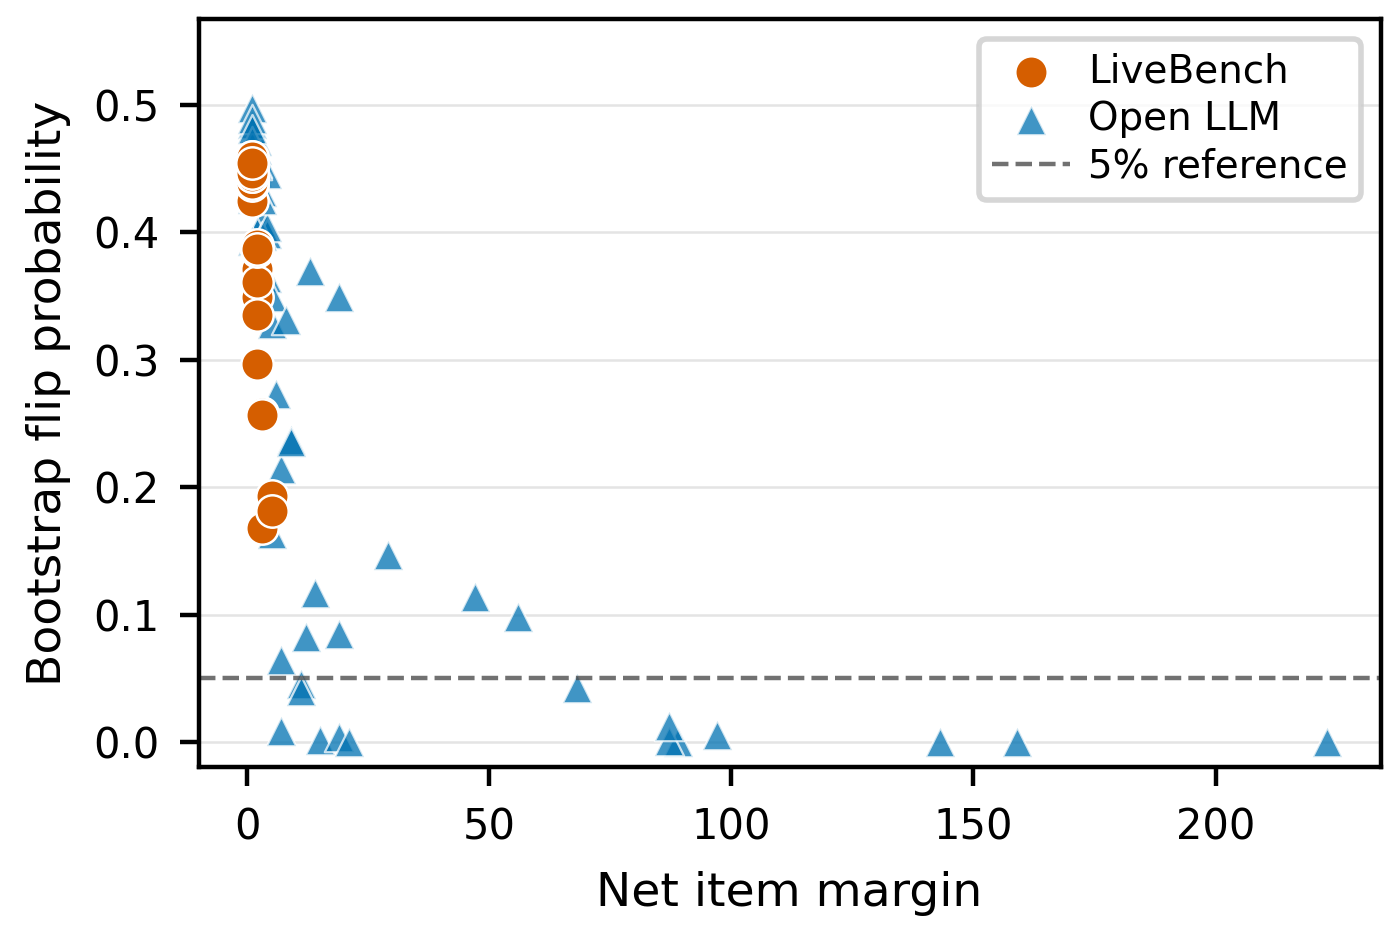
\includegraphics[width=\columnwidth]{../figures/e9_flip_vs_margin.png}
    \caption{Bootstrap flip probability vs.\ item margin across 90 rank-boundary contests. Vermillion circles: LiveBench; blue triangles: Open~LLM~Leaderboard~v1. The dashed line marks a 5\% reference threshold. Tight contests (margin $\leq 3$) are highly sample-sensitive.}
    \label{fig:flip_margin}
\end{figure}

\subsection{Per-Item Attribution on the \texttt{LCB\_generation} Top-2 Contest}
\label{sec:showcase}

The \#1~vs.~\#2 contest from \S\ref{sec:intro} (Gemini~2.5~Pro vs.\ QwQ-32B, margin~1) is a textbook fragile decision: removing any single decisive item flips it, the bootstrap flip probability is 42.5\%, and three of the seven active items favor the runner-up.
It also makes the value-function distinction concrete (Table~\ref{tab:showcase}).
Under the flip indicator the four decisive items are \emph{indistinguishable} ($\phi\approx0.33$ each) and the three counter-evidential items likewise ($\phi\approx-0.28$): the Shapley--Shubik degeneracy, now visible on real data.
The confidence value function separates them through correlation structure, while the information value function additionally weights discrimination.
The clearest contrast is the strongest versus weakest decisive item: D4 earns $\phi=0.124$, about $63\%$ of D1's $0.196$, because it is both least discriminating ($a=0.41$) and most redundant (mean $r=0.44$ with the other decisive items), so its credit is split away.
A model-population bootstrap ($B=2000$, retaining the contestants and re-estimating each $a_i$ and the correlation matrix) confirms this is signal: D4's $95\%$ CI $[.11,.14]$ lies entirely below D1's $[.16,.22]$ and D1 outranks D4 in $99.8\%$ of resamples.
The coarse structure (the redundant, low-discrimination item is worth least) is thus robust, though the fine order of the middle items is not (the full chain D1$>$D2$>$D3$>$D4 holds in $41\%$ of resamples, the adjacent CIs overlapping), so we read the result as a reliable split of pivotal from redundant decisive items, not a fully resolved ranking.
C5 is the runner-up's strongest evidence ($\phi=-0.246$, the most discriminating counter-evidential item, $a=0.99$), and the information value function accentuates the discrimination ordering.
This is per-item, structure-aware attribution that neither the flip indicator nor leave-one-out can provide.

\subsubsection{Acting on the Attribution}
The ranking changes what an auditor does next: a benchmark operator would prioritize C5 for review, not because high attribution implies a defect, but because it is the most discriminating counter-evidential item (the runner-up wins it).
The payoff is concrete: if C5 is a mislabel correcting in the winner's favor, the margin moves from 1 to 3 and flip probability drops from 42.5\% to 16.6\%; if correctly labeled, it documents an evaluated instance on which the runner-up is better without by itself establishing a broader capability difference.
An unsigned global metric would rank C5 as merely ``informative'' and give no reason to single it out, whereas signed Decision-Shapley flags it as the highest-leverage item to inspect.

\begin{table}[t]
\centering
\caption{Decision-Shapley values for the seven active items of the \texttt{LCB\_generation} \#1 vs.\ \#2 contest, with $95\%$ bootstrap CIs on $\phi_{\text{conf}}$ (model-population resampling, $B\!=\!2000$). Under the flip indicator all four decisive items collapse to $\phi\!\approx\!0.33$ and all three counter-evidential to $\approx\!-0.28$ (the Shapley--Shubik degeneracy). $\bar r$ = mean correlation with same-sign active items.}
\label{tab:showcase}
\footnotesize
\setlength{\tabcolsep}{4pt}
\begin{tabular}{@{}lrrrcr@{}}
\toprule
\textbf{Item} & $d$ & $a$ & $\bar r$ & $\phi_{\text{conf}}$ ($95\%$ CI) & $\phi_{\text{info}}$ \\
\midrule
D1 & $+1$ & 0.83 & 0.34 & $0.196$\,$[.16,.22]$ & $0.095$ \\
D2 & $+1$ & 0.80 & 0.38 & $0.191$\,$[.15,.22]$ & $0.081$ \\
D3 & $+1$ & 0.60 & 0.28 & $0.161$\,$[.13,.19]$ & $0.053$ \\
D4 & $+1$ & 0.41 & 0.44 & $0.124$\,$[.11,.14]$ & $0.024$ \\
C5 & $-1$ & 0.99 & 0.43 & $-0.246$\,$[\text{-}.27,\text{-}.21]$ & $-0.144$ \\
C6 & $-1$ & 0.76 & 0.42 & $-0.204$\,$[\text{-}.23,\text{-}.16]$ & $-0.089$ \\
C7 & $-1$ & 0.75 & 0.53 & $-0.198$\,$[\text{-}.22,\text{-}.16]$ & $-0.073$ \\
\bottomrule
\end{tabular}
\end{table}

\subsection{Validating the Attribution Against Known Ground Truth}
\label{sec:e18val}

Two objections remain: the value functions could be artifacts of their own functional form, and they might add nothing over leave-one-out or Banzhaf.
We answer both with a synthetic test whose ground truth is value-function-free.
We generate contests from a testlet 2PL model controlling two item properties, redundancy (testlet loading) and discrimination, and define each item's true decisiveness as its exact Shapley value under the \emph{population} decision probability $v^{*}(S)=\Pr_{\text{pop}}(\sum_{i\in S} d_i>0)$.
This target uses raw vote counts only, never $a_i$, $J_i$, or $C$, so scoring an estimator against it is not circular; each attribution is computed from a \emph{single} realized matrix and scored by Spearman $\rho$ over the active items, with $95\%$ bootstrap intervals over contests (Table~\ref{tab:e18}).

The result matches the specification rule of \S\ref{sec:value}.
When items differ only by redundancy (homogeneous discrimination), confidence and information are statistically tied and both clearly beat every degenerate baseline.
When items differ by discrimination, information (Eq.~\ref{eq:info}) dominates ($\rho=0.68$) while confidence falls to $\rho=-0.05$ (CI $[-0.23,0.13]$), which is consistent with zero rather than anti-correlated.
This is what the scale-invariance of confidence predicts: with no way to weight items by discrimination, it has no ranking signal to offer in this regime.
The degenerate baselines behave as Proposition~\ref{prop:degeneracy} requires.
Banzhaf is unsigned and recovers nothing ($\rho\approx0$), and the flip indicator, leave-one-out, and raw $d_i$ recover only an item's sign, plateauing at three to four times below the well-specified value function because they cannot rank items within a side.
The value functions therefore add real information over leave-one-out and Banzhaf, and since each is the better estimator in the regime where it is well-specified, the derivation and this validation agree rather than conflict.
This validation is necessarily synthetic, since ground-truth decisiveness is unobservable on real benchmarks; it establishes which value function is the correct estimator under known structure, not how often each regime arises in practice.

\begin{table}[t]
\centering
\caption{Recovery of true item decisiveness: Spearman $\rho$ with the population-decision Shapley. Each value function wins in the regime where it is well-specified; the degenerate baselines cannot rank within a side. Value-function $95\%$ bootstrap CIs over contests: redundancy conf $[.16,.36]$, info $[.14,.38]$; discrimination conf $[-.23,.13]$, info $[.60,.76]$.}
\label{tab:e18}
\footnotesize
\setlength{\tabcolsep}{5pt}
\begin{tabular}{@{}lccccc@{}}
\toprule
\textbf{Regime} & \textbf{conf.} & \textbf{info.} & \textbf{flip} & \textbf{Banz.} & \textbf{LOO} \\
\midrule
Redundancy (homog.\ $a$) & $.26$ & $.26$ & $.06$ & $.00$ & $.06$ \\
Discrim.\ (heterog.\ $a$) & $-.05$ & $.68$ & $.19$ & $.00$ & $.04$ \\
\bottomrule
\end{tabular}
\end{table}

\subsection{Does Item Discrimination Predict Decisiveness?}
\label{sec:extval}

A natural objection is circularity: Shapley values are computed from the same response matrix they purport to explain.
We therefore test a standard global item statistic, IRT discrimination / Fisher information $J_i$, against a \emph{value-function-free} measure of decisiveness, and ask whether global discrimination predicts local decisiveness.

\subsubsection{Pivotality}
For a contest we form its \emph{twin neighborhood}, the $k=\lceil\sqrt{M}\rceil$ real model pairs nearest the contest pair in ability space; the pivotality $\pi_i$ of item $i$ is the fraction of these pairs whose decision is flipped by removing item $i$ alone.
It uses no Shapley value, no value function, and no IRT fit, only leave-one-out sign flips over real model pairs.

\subsubsection{Clustered Analysis}
Contests \emph{within} a benchmark share an item set, so they are not independent; pooling and shuffling them independently is pseudoreplication and badly inflates significance (a naive pooled test returns $p=0.002$, an artifact).
We instead treat each distinct item set as one cluster, compute the within-contest Spearman $\rho(J_i,\pi_i)$ over same-sign active items, take the cluster median, and report the median across clusters; the null draws one synchronized item permutation per cluster, so it inherits the true within-cluster correlation.
This gives an effective sample of 65 independent item sets (3 LiveBench tasks, 5 whole Open~LLM benchmarks, and MMLU split into its 57 subjects), not 320 contests.

Against a no-signal floor the association looks positive but small (Table~\ref{tab:extval}, $\rho\approx0.05$--$0.09$ on Open~LLM/MMLU, null on LiveBench).
\emph{But the no-signal floor is the wrong reference.}
Because $J_i$ and $\pi_i$ are both deterministic functions of the same matrix, a positive correlation is expected purely by construction.
We quantify this with a \emph{mechanical-coupling ceiling}: for each cluster we simulate equal-discrimination (1PL/Rasch) data matched to its difficulty and ability (data with \emph{no} genuine discrimination signal), and rerun the full pipeline.

\begin{table}[t]
\centering
\caption{Discrimination $J_i$ vs.\ value-function-free pivotality $\pi_i$, clustered. Clu.\ = number of independent clusters (item sets); Obs.\ $\rho$ = observed median within-cluster Spearman correlation; Ceiling = [5th,\,50th,\,95th] percentiles of the 1PL mechanical-coupling null. Observed $\rho$ lies \emph{within or below} the ceiling in every family.}
\label{tab:extval}
\footnotesize
\setlength{\tabcolsep}{4pt}
\begin{tabular}{@{}lrrcl@{}}
\toprule
\textbf{Family} & \textbf{Clu.} & \textbf{Obs.}\,$\rho$ & \textbf{Ceiling} & \textbf{Verdict} \\
 & & & {\scriptsize[p5,\,p50,\,p95]} & \\
\midrule
LiveBench & 3 & $-.03$ & [$-.27$,\,$.01$,\,$.29$] & no signal \\
Open-LLM & 5 & $.087$ & [$.09$,\,$.25$,\,$.40$] & within band \\
MMLU subj.\ & 57 & $.052$ & [$.09$,\,$.16$,\,$.21$] & below band \\
\bottomrule
\end{tabular}
\end{table}

Under matched data with no real discrimination signal, the $J$--pivotality correlation is already $\rho\approx0.16$--$0.25$; the real data shows only $\rho\approx0.05$--$0.09$, and for MMLU it falls below the entire ceiling band.
\textbf{We therefore find no evidence that item discrimination genuinely predicts decisiveness beyond the mechanical coupling induced by sharing a response matrix.}
This conclusion uses \emph{neither} of our value functions: pivotality $\pi_i$ is value-function-free and $J_i$ is the field's standard IRT statistic, both computed without $v_{\text{conf}}$ or $v_{\text{info}}$.
It therefore cannot be an artifact of the confidence model's built-in discrimination scale-invariance (\S\ref{sec:value}): that property would, if anything, make $v_{\text{conf}}$ \emph{blind} to a discrimination effect, but the test here never invokes $v_{\text{conf}}$ in the first place.
As a one-directional robustness check, which can disconfirm the negative but not establish it, we also repeat the analysis with the information-value Shapley $\phi_i$ in place of raw $J_i$: the correlation is materially identical (MMLU: $\rho_\phi=0.068$ vs.\ $\rho_J=0.078$), so the value function does not manufacture signal, since were it doing so $\phi$ would correlate \emph{more} strongly with pivotality, not the same.

This is the empirical core of the paper.
Global IRT discrimination and local decisiveness are different things, so a global IRT statistic cannot substitute for a decision-specific attribution.
It also explains a structural blind spot of Fisher information: it is unsigned, ranking counter-evidential items (where the runner-up wins) as merely ``informative'' rather than flagging them as working against the decision; e.g.\ on ARC, counter-evidential items sit at a mean Fisher rank of 73 of 213, indistinguishable from neutral informative items.

\subsection{Report Card Artifact}
\label{sec:reportcard}

We package the analysis into a tool that accepts any per-item binary matrix and produces a decision-robustness report (JSON and HTML): the contest, bootstrap flip probability with Wilson CI, Shapley attribution with standard errors, item taxonomy, and the top decisive and counter-evidential items.
It requires no model inference, only CPU-side computation over an existing matrix, and a $200\times100$ matrix completes in under a minute on a laptop.
The implementation, reproducibility scripts, and report-card tool are publicly available at \url{https://github.com/Ubajaj1/decision-shapley}.

%======================================================================
\section{Discussion}
\label{sec:discussion}
%======================================================================

\textbf{Fragility is common.}
Top-of-leaderboard selections, especially where frontier models have converged, should routinely carry a fragility audit; here 58 of 90 contests flip with probability $>30\%$, and on contamination-resistant LiveBench all 30 analyzed exceed 16\%.

\textbf{Few items, and the wrong intuition about them.}
On \texttt{LCB\_generation}, 4 of 78 items decide \#1.
But the tempting follow-on intuition that globally high-discrimination items are the decisive ones is not supported: once mechanical coupling is accounted for, discrimination does not predict decisiveness, at least for the pivotality measure, 1PL null, and three benchmark populations we test.
This is why Decision-Shapley is necessary rather than redundant with IRT: there is no existing global statistic that tells you which items decide a contest.

\textbf{What requires Decision-Shapley, and what does not.}
The fragility findings do not need it: bootstrap flip probability, leave-one-out, and Banzhaf swing counts each suffice to show a decision is fragile, and we report the value-function-free bootstrap so those results hold independently of any Shapley choice.
What none of these can do is rank the deciding items, since by Proposition~\ref{prop:degeneracy} they give every same-sign item the same credit.
Ranking them, and separating decisive from counter-evidential items and pivotal from merely redundant ones, is what the correlation- and discrimination-aware value functions add; a practitioner deploying the ``winner'' learns that on specific counter-evidential tasks the runner-up is superior.

\textbf{Implications for benchmark design.}
Two recommendations follow: report flip probability alongside rankings, and increase item counts in competitive regions, since fragility is driven by too few differentiating items relative to tied-performance items.

\textbf{Responsible use.}
Decision leverage, global item information, and benchmark validity are distinct.
A high-magnitude attribution is a triage signal, not proof that an item is good, bad, representative, or mislabeled, and items should not be removed or reweighted solely because they are decisive for one pair.
Attribution should be used alongside annotation review, construct coverage, score gaps, and uncertainty intervals.
Likewise, flip probability is sensitivity under a stated perturbation model, not the probability that the winner is wrong: a fragile result may reflect a real but weakly supported gap, while a stable ranking may still encode systematic benchmark bias.
To discourage selective use, the headline fragility metric is independent of the Shapley value function, and per-item attribution should be reported with a value function fixed in advance and with its uncertainty.

%======================================================================
\section{Threats to Validity}
\label{sec:threats}
%======================================================================

\textbf{Mechanical coupling.}
Our pivotality $\pi_i$ and discrimination $J_i$ are both computed from the same matrix, so a nonzero association is expected by construction.
The 1PL ceiling (\S\ref{sec:extval}) bounds this; it assumes conditional item independence and is thus an imperfect, likely upward-biased estimate, but the observed correlation already lies at or below it, so our negative conclusion is the conservative one.
A higher-parameter (2PL/3PL) ceiling would not be a valid null: by giving items unequal discrimination it injects the very signal under test, raising the ceiling and making the negative conclusion only safer.
The 1PL/Rasch model is the unique no-discrimination-signal null, which is why we adopt it.
We also note a construction-level point that bears on how \S\ref{sec:extval} should be read: the confidence value function is discrimination-scale-invariant by design (a singleton is worth $\Phi(\pm1)$ regardless of $a_i$; \S\ref{sec:value}), so it could not detect a discrimination--decisiveness link even if one existed.
This is exactly why our negative result is built on the value-function-free $\pi_i$ and the raw statistic $J_i$ rather than on $v_{\text{conf}}$, and why the $\phi$-substitution above is only a check against signal inflation, not evidence for the negative.
The conclusion is also stable in the neighborhood size: sweeping $k\in\{\tfrac12,1,2\}\times\lceil\sqrt{M}\rceil$ leaves LiveBench null ($\rho$ between $-0.03$ and $0.10$) and the Open~LLM families within $0.09$--$0.14$, inside the mechanical-coupling band at every $k$.

\textbf{Bootstrap superpopulation.}
The item bootstrap treats items as exchangeable draws, an idealization for fixed benchmarks; \S\ref{sec:fragility}'s answer-flip perturbation assumes no superpopulation, preserves the fragility ordering ($\rho\geq0.85$), and is the primary check for fixed benchmarks.

\textbf{Population and contamination.}
The validation rests on three populations, two of which (Open~LLM, MMLU) are older, saturated, and partly contamination-prone; LiveBench mitigates this at the frontier but is smaller (58--155 models).

\textbf{Binary scoring and pairwise scope.}
We require binary item scores and analyze adjacent-rank contests; partial-credit scoring and all-pairs attribution are future work.

%======================================================================
\section{Conclusion}
\label{sec:conclusion}
%======================================================================

We cast leaderboard selection as a cooperative game over benchmark items and showed the obvious value functions degenerate (margin to leave-one-out, flip indicator to the Shapley--Shubik power index); two non-degenerate value functions, correlation-aware and Fisher-weighted, recover genuine per-item attribution, with the flip indicator as their formal special case.
Empirically, top-of-leaderboard decisions are frequently fragile (58 of 90 contests flip with probability $>30\%$), yet global discrimination / Fisher information does \emph{not} predict which items are decisive beyond mechanical coupling: global informativeness and local decisiveness are distinct, which is exactly why a decision-specific attribution is needed, and our report-card implementation makes such audits routine.
Future work includes partial-credit value functions, all-pairs attribution, and live-leaderboard integration.

\bibliographystyle{IEEEtran}

\begin{thebibliography}{20}

\bibitem{alzahrani2024benchmarks}
N.~Alzahrani et al.,
``When benchmarks are targets: Revealing the sensitivity of large language model leaderboards,''
in \emph{Proc.\ ACL}, 2024, pp.~13787--13805.

\bibitem{miller2024adding}
E.~Miller,
``Adding error bars to evals: A statistical approach to language model evaluations,''
\emph{arXiv:2411.00640}, 2024.

\bibitem{burnell2023rethink}
R.~Burnell et al.,
``Rethink reporting of evaluation results in AI,''
\emph{Science}, vol.~380, no.~6641, pp.~136--138, 2023.

\bibitem{card2020power}
D.~Card, P.~Henderson, U.~Khandelwal, R.~Jia, K.~Mahowald, and D.~Jurafsky,
``With little power comes great responsibility,''
in \emph{Proc.\ EMNLP}, 2020.

\bibitem{lordnovick1968}
F.~M.~Lord and M.~R.~Novick,
\emph{Statistical Theories of Mental Test Scores},
Addison-Wesley, 1968.

\bibitem{lundberg2017shap}
S.~M.~Lundberg and S.-I.~Lee,
``A unified approach to interpreting model predictions,''
in \emph{Proc.\ NeurIPS}, 2017.

\bibitem{kipnis2025metabench}
A.~Kipnis et al.,
``metabench --- A sparse benchmark of reasoning and knowledge in large language models,''
in \emph{Proc.\ ICLR}, 2025.

\bibitem{polo2024tinybenchmarks}
F.~Maia~Polo, L.~Weber, L.~Choshen, Y.~Sun, G.~Xu, and M.~Yurochkin,
``tinyBenchmarks: Evaluating LLMs with fewer examples,''
in \emph{Proc.\ ICML}, 2024.

\bibitem{fromskills2024}
G.~Maimon, A.~Cohen, G.~Vishne, S.~Ravfogel, and R.~Tsarfaty,
``From benchmarks to skills: Low-rank factors for LLM evaluation,''
\emph{arXiv:2507.20208}, 2025.

\bibitem{perlitz2024efficient}
Y.~Perlitz et al.,
``Efficient benchmarking (of language models),''
in \emph{Proc.\ NAACL}, 2024.

\bibitem{shapley1953value}
L.~S.~Shapley,
``A value for $n$-person games,''
in \emph{Contributions to the Theory of Games II}, pp.~307--317, Princeton Univ.\ Press, 1953.

\bibitem{shapleyshubik1954}
L.~S.~Shapley and M.~Shubik,
``A method for evaluating the distribution of power in a committee system,''
\emph{American Political Science Review}, vol.~48, no.~3, pp.~787--792, 1954.

\bibitem{banzhaf1965}
J.~F.~Banzhaf,
``Weighted voting doesn't work: A mathematical analysis,''
\emph{Rutgers Law Review}, vol.~19, pp.~317--343, 1965.

\bibitem{ghorbani2019data}
A.~Ghorbani and J.~Zou,
``Data Shapley: Equitable valuation of data for machine learning,''
in \emph{Proc.\ ICML}, 2019.

\bibitem{jia2019efficient}
R.~Jia et al.,
``Towards efficient data valuation based on the Shapley value,''
in \emph{Proc.\ AISTATS}, 2019.

\bibitem{liang2023helm}
P.~Liang et al.,
``Holistic evaluation of language models,''
\emph{Transactions on Machine Learning Research}, 2023.

\bibitem{zheng2024chatbot}
L.~Zheng et al.,
``Judging LLM-as-a-Judge with MT-bench and Chatbot Arena,''
in \emph{Proc.\ NeurIPS Datasets and Benchmarks Track}, 2023.

\bibitem{efron1979bootstrap}
B.~Efron,
``Bootstrap methods: Another look at the jackknife,''
\emph{The Annals of Statistics}, vol.~7, no.~1, pp.~1--26, 1979.

\bibitem{livebench}
C.~White et al.,
``LiveBench: A challenging, contamination-limited LLM benchmark,''
\emph{arXiv:2406.19314}, 2024.

\bibitem{jain2024livecodebench}
N.~Jain, K.~Han, A.~Gu, W.-D.~Li, F.~Yan, T.~Zhang, S.~Wang, A.~Solar-Lezama, K.~Sen, and I.~Stoica,
``LiveCodeBench: Holistic and contamination free evaluation of large language models for code,''
\emph{arXiv:2403.07974}, 2024.

\end{thebibliography}

\end{document}
